%=========================================================================
%  Foundational Amplitudes -- progress report to collaborators
%  Joaquin Iturriza Ramirez
%  Compile (twice):  pdflatex -interaction=nonstopmode main.tex
%=========================================================================
\documentclass[aspectratio=169,10pt]{beamer}

\usepackage[T1]{fontenc}
\usepackage[utf8]{inputenc}
\usepackage{helvet}
\renewcommand{\familydefault}{\sfdefault}
\usefonttheme{professionalfonts}
\usepackage{graphicx}
\usepackage{amsmath,amssymb}
\usepackage{booktabs}
\usepackage{multirow}
\usepackage{xcolor}
\usepackage{tikz}
\usetikzlibrary{positioning,fit,backgrounds,calc}

% local figs first, then the project figure trees
\graphicspath{{figs/}{../../docs/figs/}{../../plots/}{../../analysis/hpo_optima/}}

%---------- colours / theme (same as the CSI talk) ------------------------
\definecolor{navy}{RGB}{38,38,110}
\definecolor{good}{RGB}{20,120,40}
\definecolor{warn}{RGB}{190,70,20}
\definecolor{tfemb}{HTML}{F8CECC}
\definecolor{tfatt}{HTML}{FFE6CC}
\definecolor{tfnrm}{HTML}{FFF2CC}
\definecolor{tfff}{HTML}{DAE8FC}

\setbeamercolor{frametitle}{fg=navy}
\setbeamercolor{title}{fg=navy}
\setbeamercolor{structure}{fg=navy}
\setbeamercolor{itemize item}{fg=navy}
\setbeamercolor{itemize subitem}{fg=navy!60}
\setbeamertemplate{navigation symbols}{}
\setbeamertemplate{itemize item}{\textbullet}
\setbeamertemplate{itemize subitem}{\textendash}

\setbeamertemplate{frametitle}{%
  \vskip0.6em\hbox{\hspace{0.2em}\usebeamerfont{frametitle}\insertframetitle}%
  \vskip0.12em\hbox{\hspace{0.2em}\textcolor{navy}{\rule{0.965\paperwidth}{0.8pt}}}\vskip0.2em}

\setbeamertemplate{footline}{%
  \hfill\usebeamerfont{normal text}\color{gray}\scriptsize\insertframenumber\hspace{1em}\vspace{0.6em}}

\setbeamerfont{frametitle}{size=\Large,series=\bfseries}

% helper macros
\newcommand{\takeaway}[1]{\vfill\begin{center}\colorbox{navy!8}{\parbox{0.9\textwidth}{\centering\textcolor{navy}{\textbf{#1}}}}\end{center}\vskip0.3em}
\newcommand{\Amp}{\ensuremath{|\mathcal{M}|^2}}
\newcommand{\vlnr}{\ensuremath{\mathcal{L}^{\mathrm{val}}_{0}}}
\newcommand{\win}{\textcolor{good}{\textbf{kept}}}
\newcommand{\lose}{\textcolor{warn}{\textbf{discarded}}}
\newcommand{\secdiv}[3]{%
  \begin{frame}[plain]\centering\vfill
  {\color{navy}\Large\bfseries #1}\\[0.6em]{\large #2}\\[0.4em]
  {\footnotesize\color{gray} #3}\vfill\end{frame}}

\title{A foundation model for scattering amplitudes: progress report}
\author{Joaqu\'in Iturriza Ramirez}

%=========================================================================
\begin{document}

%---------------------------------------------------------------- TITLE
\begin{frame}[plain]
  \vfill
  \begin{center}
    {\Large\bfseries\color{navy} A foundation model for scattering amplitudes\\[0.2em] progress report}\\[1.4em]
    {\large Joaqu\'in Iturriza Ramirez}\\[0.4em]
    {\footnotesize LPNHE, Sorbonne Universit\'e / CNRS-IN2P3}\\[1.2em]
    {\footnotesize\color{gray} Collaboration meeting \quad\textbar\quad July 2026}\\[0.6em]
    {\scriptsize\color{gray} trained on the Jean Zay supercomputer (IDRIS)}
  \end{center}
  \vfill
\end{frame}

%---------------------------------------------------------------- IDEA
\begin{frame}{The idea: one model for all amplitudes}
  \begin{columns}[T]
    \begin{column}{0.52\textwidth}
      \footnotesize
      \begin{itemize}
        \item A surrogate replaces the per-point matrix-element call:
          \begin{center}\fbox{particle momenta $\longrightarrow$ \Amp}\end{center}
        \item Until now: \textbf{one network per process}. Wasteful --- the networks share no physics, each starts from zero.
        \item \textbf{This project:} a \emph{single} Lorentz-equivariant transformer trained \textbf{jointly} on many processes
          ($ee\!\to\!WW$, $t\bar t$, $u\bar u(g)$, $\gamma\gamma(\gamma)$, \dots up to \textbf{448 datasets}), tree \emph{and} loop level.
        \item Then \textbf{fine-tuned} to any new process or perturbative order with a fraction of the data.
      \end{itemize}
    \end{column}
    \begin{column}{0.44\textwidth}
      \centering
      \includegraphics[width=0.85\linewidth]{amp_surface_pts.png}\\[0.2em]
      {\scriptsize\color{gray} \Amp{} over a phase-space slice; \textcolor{warn}{dots} $=$ training samples.}
    \end{column}
  \end{columns}
  \takeaway{Learn the physics once, reuse it everywhere: new process $=$ cheap fine-tune, not a new model.}
\end{frame}

%---------------------------------------------------------------- OUTLINE
\begin{frame}{Outline}
  \footnotesize
  \begin{enumerate}
    \item \textbf{The model} --- what a transformer is, how LLoCa makes it Lorentz-equivariant.
    \item \textbf{What the network is fed} --- beyond the four-momenta: quantum numbers, couplings, off-shellness, \dots
    \item \textbf{How we decide what stays} --- the A/B protocol, and every feature we accepted or discarded.
    \item \textbf{Results} --- scaling laws, transfer to one-loop targets, the 448-process run.
    \item \textbf{Open problems and next steps.}
  \end{enumerate}
\end{frame}

%================================================================ MODEL
\secdiv{Part 1}{The model}{a Lorentz-equivariant transformer, briefly}

%---------------------------------------------------------------- TRANSFORMER
\begin{frame}{What is a transformer? (30-second version)}
  \begin{columns}[c]
    \begin{column}{0.55\textwidth}
      \footnotesize
      \begin{itemize}
        \item A neural network for \textbf{sets} of objects --- here, the \textbf{particles of one event}.
        \item Core operation, \textbf{self-attention}: each particle builds its representation by mixing information from \emph{all other particles in the event}, with learned weights (``which particles matter to me?'').
        \item Naturally handles \textbf{variable particle number} and is blind to the \textbf{ordering} of the particles --- exactly the structure of an event.
        \item Ours: 8 attention blocks; events are packed together and a mask keeps particles attending only \emph{within their own event}.
      \end{itemize}
    \end{column}
    \begin{column}{0.45\textwidth}
      \centering
      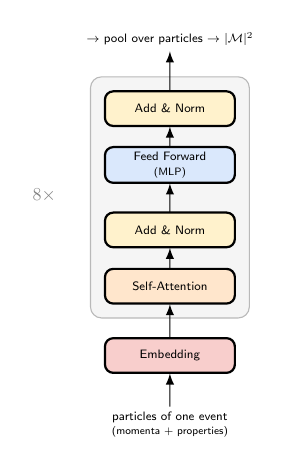
\begin{tikzpicture}[scale=0.55,transform shape,font=\footnotesize,>=latex,
        blk/.style={draw=black,thick,rounded corners=3pt,minimum width=30mm,minimum height=8mm,align=center},
        emb/.style={blk,fill=tfemb},att/.style={blk,fill=tfatt},nrm/.style={blk,fill=tfnrm},ff/.style={blk,fill=tfff},
        lbl/.style={align=center}]
        \node[lbl] (in) at (0,-1.3) {particles of one event\\{\scriptsize(momenta $+$ properties)}};
        \node[emb] (e) at (0,0.3) {Embedding};
        \node[att] (a) at (0,1.9) {Self-Attention};
        \node[nrm] (n1) at (0,3.2) {Add \& Norm};
        \node[ff]  (f) at (0,4.7) {Feed Forward\\{\scriptsize(MLP)}};
        \node[nrm] (n2) at (0,6.0) {Add \& Norm};
        \node[lbl] (out) at (0,7.6) {$\to$ pool over particles $\to$ \Amp};
        \draw[->](in)--(e);\draw[->](e)--(a);\draw[->](a)--(n1);\draw[->](n1)--(f);\draw[->](f)--(n2);\draw[->](n2)--(out);
        \begin{scope}[on background layer]
          \node[draw=gray!55,rounded corners,fill=gray!8,fit=(a)(n2),inner sep=5pt] {};
        \end{scope}
        \node[gray] at (-2.9,4.0) {\large$8\times$};
      \end{tikzpicture}\\[0.2em]
      {\scriptsize\color{gray} encoder-only transformer (Vaswani et al.\ 2017).}
    \end{column}
  \end{columns}
  \takeaway{A transformer fits amplitudes because an event is an unordered, variable-length set of particles.}
\end{frame}

%---------------------------------------------------------------- LLOCA
\begin{frame}{LLoCa: exact Lorentz equivariance, cheaply}
  \begin{columns}[T]
    \begin{column}{0.46\textwidth}
      \footnotesize
      \begin{itemize}
        \item Amplitudes respect \textbf{Lorentz symmetry}; a network that has it built in does not waste capacity re-learning it.
        \item \textbf{LLoCa} (Lorentz Local Canonicalization, 2505.20280): a small ``frames'' network predicts, for each particle, its own \textbf{local Lorentz frame} $\Lambda_i$, equivariantly.
        \item Momenta mapped into their own frames become \textbf{Lorentz-invariant numbers}; a plain transformer processes them; the whole chain is \emph{exactly} equivariant.
        \item Because the backbone is an ordinary transformer, it is $\sim$\textbf{20$\times$ fewer FLOPs} than fully-tensorial equivariant nets (L-GATr) --- and, as we'll see, also \emph{more accurate} at equal budget.
        \item Trained with \textbf{$\mu$P}: hyperparameters tuned at small size stay valid at any larger size (backup).
      \end{itemize}
    \end{column}
    \begin{column}{0.54\textwidth}
      \centering
      \includegraphics[width=\linewidth]{lloca_white.png}\\[0.4em]
      {\scriptsize\color{gray} LLoCa: learn each particle's local frame; any backbone becomes Lorentz-equivariant.}
    \end{column}
  \end{columns}
  \takeaway{Exact Lorentz symmetry at the cost of a plain transformer.}
\end{frame}

%================================================================ INPUTS
\secdiv{Part 2}{What the network is fed}{beyond the four-momenta}

%---------------------------------------------------------------- ENCODING
\begin{frame}{Particles are their quantum numbers, not their names}
  \footnotesize
  \begin{columns}[T]
    \begin{column}{0.55\textwidth}
      \begin{itemize}
        \item Each particle enters as its momentum \textbf{plus an 8-component physical property vector}:
        \[ \bigl[\,Q,\ \mathrm{spin},\ \log_{10} m,\ T_3,\ B,\ L,\ \mathrm{color},\ C_2(R)\,\bigr] \]
        \item Spin and color are \textbf{labels, not magnitudes} (spin-1 is not ``twice'' spin-$\tfrac12$) $\Rightarrow$ one-hot encoded; a flag marks exactly-massless particles.
        \item \textbf{Why not a particle dictionary} (one-hot ID)? A dictionary model \emph{cannot even represent} a particle it never saw.
      \end{itemize}
    \end{column}
    \begin{column}{0.45\textwidth}
      \begin{itemize}
        \item With quantum numbers, a frozen pretrained model already predicts \textbf{entirely unseen processes zero-shot}: MSE $0.22$--$0.51$ on the standardized target, vs.\ $1.0$ for the trivial constant predictor.
        \item Adding a new particle or a 9th quantum number \textbf{never forces retraining} the transformer --- the input size depends on the number of \emph{properties}, not the vocabulary.
      \end{itemize}
    \end{column}
  \end{columns}
  \takeaway{Encoding particles by physics, not identity, is what makes transfer to new processes possible at all.}
\end{frame}

%---------------------------------------------------------------- EXTRA INPUTS
\begin{frame}{The extra inputs: what the momenta cannot tell you}
  \footnotesize
  Per-dataset physics that is \emph{not} a function of the external momenta is broadcast to every particle as extra scalars:
  \vskip0.4em
  \begin{itemize}
    \item \textbf{Coupling order} $[n_{\rm loops},\ \alpha_s\text{-power}]$: LO $=[0,0]$, full NLO $=[1,1]$, virtual-only $=[1,0]$.\\
      {\color{gray} $\Rightarrow$ mixing perturbative orders in one model needs \emph{no architecture change}.}
    \item \textbf{Coupling value} $\log\alpha$ --- for datasets scanning the coupling strength.
    \item \textbf{Internal propagator masses} (scanned $Z$, top, Higgs), supplied as the per-event \textbf{off-shellness} $s_{\rm prop}-M^2$: the distance of the event to the pole of an \emph{internal} line that never appears among the external momenta.
    \item \textbf{Feynman-diagram graph} of the process, embedded by a graph encoder {\color{gray}(tried --- see the ablations)}.
  \end{itemize}
  \vskip0.3em\relax
  Plus a preprocessing that matters: \Amp{} spans $\sim$13 orders of magnitude and can be negative at one loop $\Rightarrow$ log (or signed-log) compression $+$ standardization, resolved \textbf{per process}.
  \takeaway{Guiding principle (verified below): a feature helps exactly when it supplies something the external momenta cannot recover.}
\end{frame}

%================================================================ AB TESTS
\secdiv{Part 3}{What survived and what didn't}{every feature A/B-tested, accepted or discarded on evidence}

%---------------------------------------------------------------- PROTOCOL
\begin{frame}{How each decision is made: the A/B protocol}
  \footnotesize
  \begin{columns}[T]
    \begin{column}{0.55\textwidth}
      \begin{enumerate}
        \item The baseline is the \textbf{best run of a short hyperparameter sweep} (Bayesian optimization), never a single arbitrary run.
        \item Try the new feature \textbf{at the baseline's best hyperparameters}: if it already wins, done.
        \item If not, give the feature \textbf{its own equal sweep} and compare best-vs-best.
      \end{enumerate}
    \end{column}
    \begin{column}{0.45\textwidth}
      \begin{itemize}
        \item Metric, always: \vlnr{} $=$ best \textbf{non-regularized validation loss} on the log-amplitude --- the regularization strength is itself a tuned knob, so regularized losses are not comparable.
        \item If a feature changes the preprocessing, losses are re-based to the same scale before comparing.
      \end{itemize}
    \end{column}
  \end{columns}
  \takeaway{Fair (both sides get tuned hyperparameters) and frugal (stop early when the cheap test already decides).}
\end{frame}

%---------------------------------------------------------------- PREPROCESSING
\begin{frame}{Accepted: per-process preprocessing (a genuine bug fix)}
  \footnotesize
  \begin{itemize}
    \item One loop-level dataset has \emph{negative} amplitudes (interference) $\Rightarrow$ a single \emph{global} transform is forced to signed-log for \textbf{everyone}.
    \item But signed-log only compresses $|a|\gg1$, and every $\Amp\ll1$: targets stay in \emph{linear} scale, per-process spreads of $8$--$30$ (up to $1.2\times10^4$) --- most processes simply \textbf{fail to train}.
    \item Fix: resolve the transform and its $(\mu,\sigma)$ \textbf{per process} (in the 448-dataset run: 416 get log, 32 signed-log).
  \end{itemize}
  \vskip0.3em
  \centering
  \begin{tabular}{@{}lcc@{}}
    \toprule
     & global transform & per-process \\
    \midrule
    spread of the preprocessed target & $282$ & $\mathbf{1.06}$ \\
    median relative error & --- & $\sim\mathbf{6\times}$ lower \\
    \bottomrule
  \end{tabular}
  \takeaway{Per-process preprocessing is the validated default; it also de-sensitized every subsequent sweep.}
\end{frame}

%---------------------------------------------------------------- LOSS
\begin{frame}{Accepted: aggregate the joint loss in log-space}
  \footnotesize
  \begin{itemize}
    \item Training on $P$ processes at once: how to combine the per-process errors $m_p$ into one loss?
    \item Processes of different final-state multiplicity plateau at wildly different error scales ($\sim\!10^{-6}$ for $2\!\to\!2$ vs.\ $\sim\!10^{-2}$ for $2\!\to\!4$): an \textbf{arithmetic mean} is owned by the few hard processes and the easy ones stop improving.
    \item Adopted: the \textbf{geometric mean} $\exp\bigl(\tfrac1P\sum_p \ln m_p\bigr)$ --- a 10\% \emph{relative} gain counts the same for every process, so all keep scaling.
  \end{itemize}
  \vskip0.4em
  \textbf{Also tested here --- and \lose: an adaptive ``balanced'' sampler} that re-weights batch composition toward processes still improving (plateau detection via local scaling exponents).
  \begin{itemize}
    \item Best-vs-best A/B on 8 processes: plain uniform sampling $8.1\times10^{-8}$ vs.\ balanced $2.6\times10^{-7}$ --- the simple option wins $3\times$.
    \item Perturbing the sampling dynamics costs more than it gains; kept only as an option for few, very unbalanced datasets.
  \end{itemize}
  \takeaway{Geometric-mean loss: accepted. Adaptive sampler: discarded --- uniform sampling wins.}
\end{frame}

%---------------------------------------------------------------- LEVERS
\begin{frame}{The physics-feature A/B campaign}
  \footnotesize
  One feature toggled per test, matched hyperparameters, targeted processes:
  \vskip0.2em
  \centering
  \begin{tabular}{@{}llrrl@{}}
    \toprule
    Feature & test & off & on & verdict \\
    \midrule
    coupling $\log\alpha$ (unrecoverable case) & $ee\,u\bar u ggg$, pooled std & $0.0573$ & $0.0031$ & \textbf{win 18$\times$} \\
    coupling $\log\alpha$ (recoverable case) & same, per-dataset std & $0.0049$ & $0.0046$ & neutral \\
    external mass from momenta & near-threshold $t\bar t$ & $2.1\text{e-}5$ & $1.7\text{e-}5$ & redundant \\
    internal mass as a raw scalar & $M_Z$ scan, $ee\,\mu\mu$ & $0.0756$ & $0.0795$ & \textcolor{warn}{\textbf{fails}} \\
    resonance $\sqrt s - M$ ($s$-channel only) & $M_Z$ scan & $0.0819$ & $1.8\text{e-}5$ & win 4500$\times$ \\
    \textbf{off-shellness} $s_{\rm prop}-M^2$ (general) & $M_Z$ scan & $0.0763$ & $9.4\text{e-}5$ & \textbf{win 810$\times$, adopted} \\
    \bottomrule
  \end{tabular}
  \vskip0.5em
  \raggedright
  \begin{itemize}
    \item The pattern is one principle: a feature wins \textbf{iff} it supplies what the momenta cannot recover (a coupling, an internal mass), \emph{in a usable form} --- the raw mass scalar fails, the kinematic distance-to-pole succeeds.
    \item Off-shellness adopted over the (slightly better) resonance form: it generalizes to $t$-channel and to the top/Higgs propagators instead of hard-coding one topology.
  \end{itemize}
\end{frame}

%---------------------------------------------------------------- FLAGSHIP
\begin{frame}{Flagship result: off-shellness conditioning, 50$\times$}
  \begin{columns}[T]
    \begin{column}{0.42\textwidth}
      \footnotesize
      \begin{itemize}
        \item Confirmation in the regime that matters: \textbf{44 datasets} spanning the $Z$, top and Higgs resonances, full data, fiducial cuts, 30k steps.
        \item Off-shellness $s_{\rm prop}-M^2$ for the internal $Z/t/H$ lines, fed directly to the transformer.
        \item Best validation loss: $0.268 \to 0.0053$ --- \textbf{50$\times$ better}.
        \item On by default in all production runs since.
      \end{itemize}
    \end{column}
    \begin{column}{0.58\textwidth}
      \centering
      \includegraphics[width=\linewidth]{levers_offshell_ab.pdf}\\[0.1em]
      {\scriptsize\color{gray} validation loss vs.\ training step, feature off vs.\ on.}
    \end{column}
  \end{columns}
  \takeaway{Telling the network how far each event is from the internal poles is the single largest gain found.}
\end{frame}

%---------------------------------------------------------------- ARCH AB
\begin{frame}{Architecture shoot-out: LLoCa vs.\ L-GATr}
  \footnotesize
  Three maintained Lorentz-equivariant architectures at matched size ($\approx$1.6M parameters), compared at \textbf{equal compute} and \textbf{equal wall-time} (each with its own tuned sweep --- a step-matched comparison would be meaningless at 20$\times$ different cost/step):
  \vskip0.3em
  \centering
  \begin{tabular}{@{}lrr@{\hskip 2.2em}rr@{}}
    \toprule
     & \multicolumn{2}{c}{cost} & \multicolumn{2}{c}{best val.\ loss} \\
    \cmidrule(r){2-3}\cmidrule(l){4-5}
    Model & params & GFLOP/step & eq.\ compute & eq.\ time \\
    \midrule
    \textbf{LLoCa} & $1.61$M & $\mathbf{48.8}$ & $\mathbf{5.98\times10^{-3}}$ & $\mathbf{5.98\times10^{-3}}$ \\
    L-GATr slim & $1.57$M & $74.3$ & $2.00\times10^{-2}$ & $2.21\times10^{-2}$ \\
    L-GATr & $1.64$M & $999.2$ & $5.29\times10^{-2}$ & $4.23\times10^{-2}$ \\
    \bottomrule
  \end{tabular}
  \vskip0.5em
  \raggedright
  \begin{itemize}
    \item LLoCa is simultaneously the \textbf{cheapest} ($20\times$ fewer FLOPs/step than L-GATr) and the \textbf{most accurate} ($3$--$9\times$ lower loss) at fixed budget.
  \end{itemize}
  \takeaway{LLoCa is the default by measurement, not convention.}
\end{frame}

%---------------------------------------------------------------- ENCODING AB
\begin{frame}{Encoding ablations: small-scale hints, settled at full scale}
  \footnotesize
  Optional channels of the particle encoding, swept $+$ 5-seed confirmed on 25 processes, then \textbf{re-tested one-factor-out at 448 datasets} (the decisive column: geometric-mean loss over the 390 processes that converge in every arm):
  \vskip0.3em
  \centering
  \begin{tabular}{@{}llll@{}}
    \toprule
    Channel & small-scale (25 proc) & full-scale (448 sets) & verdict \\
    \midrule
    one-hot spin $+$ massless flag $+$ std. & clear win & --- & \win \\
    one-hot color & $+12\%$ (within noise) & removing costs $+17\%$ & \win \\
    MLP embedder (vs.\ linear) & $+24\%$ (within noise) & not load-bearing & \lose \\
    diagram-graph encoder & motivated, kept on & removing \textbf{gains} $35\%$ & \lose \\
    off-shellness & win (prev.\ slide) & removing costs $+46\%$ & \win \\
    \bottomrule
  \end{tabular}
  \vskip0.5em
  \raggedright
  \begin{itemize}
    \item Lesson: short small-data A/Bs can mislead in both directions --- color's ``$+12\%$ cost'' was undertraining noise (it actually helps), while the diagram encoder, plausible on paper, \emph{actively hurts} at scale.
    \item Adopted production encoding: quantum numbers with one-hot spin/color, massless flag, linear embedder, off-shellness --- \textbf{no diagram encoder}.
  \end{itemize}
\end{frame}

%---------------------------------------------------------------- PAIR BIAS
\begin{frame}{Tested and not adopted: pairwise attention bias}
  \footnotesize
  \begin{itemize}
    \item Idea: put the off-shellness signal \emph{where the pair correlation lives} --- each internal propagator's $s-m^2$ shifts the attention weights of the particle pairs it resonates with.
    \item \textbf{It works on its targets}: the hardest (``stuck'') processes improve --- e.g.\ Bhabha $0.81\!\to\!0.012$, $ee\!\to\!ZH$ $0.31\!\to\!0.0009$, $ee\!\to\!\gamma\gamma$ $0.41\!\to\!0.009$; fewest failing processes of any arm.
    \item \textbf{But the already-converged bulk pays a robust 30--50\% tax}, and no variant (logit cap, propagator-identity features, halved learning rate) removes it $\Rightarrow$ the cost is design-intrinsic, and under the 448-process aggregate the verdict is a \textbf{net loss}.
    \item Diagnosis: one globally-shared bias cannot serve 448 processes whose gradient scales differ by $10^4$ --- the fix belongs in the loss aggregation (next steps), after which this can return as a \emph{gated} rescue for stuck processes.
  \end{itemize}
  \takeaway{A clean negative: demonstrated rescues on the hard tail, rejected because the bulk pays for them.}
\end{frame}

%---------------------------------------------------------------- LR LAW
\begin{frame}{A by-product: how the learning rate must be set (422 sweeps)}
  \begin{columns}[T]
    \begin{column}{0.42\textwidth}
      \footnotesize
      \begin{itemize}
        \item Harvesting all converged hyperparameter sweeps ($422$ of $771$) gives an \emph{optimization law}:
        \item The optimal learning rate is \textbf{flat across model width} ($\mu$P works: tune small, reuse large) \dots
        \item \dots but follows an \textbf{inverted-U in training length}, peaking at $\approx$3000 steps regardless of dataset size --- an optimizer timescale, not convergence.
        \item Practical payoff: new sweeps are centred on the measured surface and search $\pm\tfrac12$ decade instead of 4 decades $\Rightarrow$ \textbf{half the trial budget} at equal resolution.
      \end{itemize}
    \end{column}
    \begin{column}{0.58\textwidth}
      \centering
      \includegraphics[width=\linewidth]{lr_vs_iterations_by_regime.pdf}\\[0.1em]
      {\scriptsize\color{gray} best learning rate vs.\ training steps: rises $\sim t^{+0.5}$, peaks at $\sim$3k, falls $\sim t^{-0.55}$.}
    \end{column}
  \end{columns}
  \takeaway{Hyperparameter search is now seeded from a measured law, not a flat prior.}
\end{frame}

%================================================================ RESULTS
\secdiv{Part 4}{Results}{scaling, transfer, and the 448-process run}

%---------------------------------------------------------------- SCALING
\begin{frame}{Scaling: error vs.\ compute is a power law set by the physics}
  \begin{columns}[T]
    \begin{column}{0.40\textwidth}
      \footnotesize
      \begin{itemize}
        \item Held-out loss vs.\ training compute follows $L(C)=A\,C^{-\alpha_C}+L_\infty$.
        \item The exponent \textbf{tracks the final-state multiplicity}: $\alpha_C\approx1.7$--$2.2$ ($2\!\to\!2$), $1.1$--$1.3$ ($2\!\to\!3$), $0.96$ ($2\!\to\!4$) --- following the bound $\alpha=4/\mathrm{DOF}$, $\mathrm{DOF}=3n_f-4$.
        \item The exponent is \textbf{width-independent}: model size enters only through compute ($\mu$P at work).
        \item $\Rightarrow$ the cost of a precision target is \textbf{predictable from the process alone}, before training.
      \end{itemize}
    \end{column}
    \begin{column}{0.60\textwidth}
      \centering
      \includegraphics[width=0.94\linewidth]{alpha_vs_multiplicity_overlay.pdf}\\[0.1em]
      {\scriptsize\color{gray} fitted exponents per process family vs.\ the $4/\mathrm{DOF}$ bound (grey wedge); stars $=$ fine-tuned one-loop targets.}
    \end{column}
  \end{columns}
  \takeaway{Harder final states learn more slowly per FLOP, by a predictable amount.}
\end{frame}

%---------------------------------------------------------------- TRANSFER
\begin{frame}{Transfer: fine-tuning beats from-scratch, and never plateaus}
  \begin{columns}[T]
    \begin{column}{0.40\textwidth}
      \footnotesize
      \begin{itemize}
        \item Targets: \textbf{one-loop (NLO-virtual)} $ee\!\to\!u\bar u$ and $ee\!\to\!t\bar t$, fine-tuned from jointly-pretrained foundations vs.\ trained from scratch.
        \item Same scaling exponent --- but the fine-tuned curve is \textbf{strictly lower at every budget} and, decisively, \textbf{keeps descending} where from-scratch flattens: 1--2 orders of magnitude lower floor.
        \item Holds even for a foundation that \textbf{never saw the target process at any order} $\Rightarrow$ genuine transfer of shared structure, not memorization.
      \end{itemize}
    \end{column}
    \begin{column}{0.60\textwidth}
      \centering
      \includegraphics[width=\linewidth]{compute_scan_eettbar_wt.pdf}\\[0.1em]
      {\scriptsize\color{gray} $ee\!\to\!t\bar t$ one-loop: test error vs.\ wall-time, one panel per dataset size ($10^3$--$10^6$ events); from-scratch vs.\ fine-tunes from several foundations.}
    \end{column}
  \end{columns}
  \takeaway{Pretraining pays off exactly where it should: little data, new process, higher order.}
\end{frame}

%---------------------------------------------------------------- FT METHODS
\begin{frame}{How to fine-tune: full retraining wins}
  \footnotesize
  Five fine-tuning methods compared on $ee\!\to\!t\bar t$ one-loop (best val.\ loss at three budgets):
  \vskip0.3em
  \centering
  \begin{tabular}{@{}lrrrrr@{}}
    \toprule
    steps & \textbf{full (layer-decay)} & reset-head & freeze & EWC & LoRA \\
    \midrule
    $400$   & $\mathbf{3.2\times10^{-5}}$ & $5.4\times10^{-4}$ & $5.4\times10^{-4}$ & $5.9\times10^{-4}$ & $1.1\times10^{-3}$ \\
    $4000$  & $\mathbf{5.5\times10^{-7}}$ & $1.5\times10^{-6}$ & $1.6\times10^{-6}$ & $5.7\times10^{-6}$ & $4.8\times10^{-6}$ \\
    $40000$ & $\mathbf{2.7\times10^{-9}}$ & $2.7\times10^{-9}$ & $4.8\times10^{-9}$ & $1.9\times10^{-8}$ & $8.9\times10^{-9}$ \\
    \bottomrule
  \end{tabular}
  \vskip0.5em
  \raggedright
  \begin{itemize}
    \item Full retraining with a per-layer learning-rate decay is best at \textbf{every intermediate budget}, often 1--2 orders of magnitude ahead ($\sim$10$\times$ faster in wall-time to a given error); the methods only meet at the shared floor.
    \item Parameter-efficient methods (LoRA, freezing) buy nothing here --- our models are small enough to just retrain.
  \end{itemize}
  \takeaway{Default adopted: full fine-tune with layer decay, learning rate $\approx$ the pretraining one.}
\end{frame}

%---------------------------------------------------------------- BIG RUN
\begin{frame}{The 448-process run: what a joint model actually learns}
  \footnotesize
  First full-scale campaign: \textbf{448 datasets} ($10^5$ events each --- coupling scans, mass scans, plain processes), one model, batch 16384.
  \begin{itemize}
    \item Median per-process loss $2\times10^{-4}$ --- the bulk trains well. But \textbf{50/448 datasets fail}, the \emph{same ones in every trial}: systematic, not noise.
  \end{itemize}
  \vskip0.2em
  \centering
  \begin{tabular}{@{}lrrl@{}}
    \toprule
    category & failing & total & why \\
    \midrule
    coupling-scan variants & $0$ & $336$ & all learn, down to $10^{-4}$ \\
    narrow-window $M_Z$-scans & $3$ & $60$ & (only the widest windows) \\
    $m_t/m_H/M_Z^{4\ell}$ scan families & $32$ & $32$ & resonance in an \emph{internal} invariant mass \\
    plain wide-range processes & $15$ & $20$ & $Z$ pole is $0.3\%$ of the $\sqrt s$ window \\
    \bottomrule
  \end{tabular}
  \vskip0.5em
  \raggedright
  Two identified mechanisms:
  \begin{itemize}
    \item \textbf{Resonance needles}: flat phase-space sampling barely populates the poles; the same processes with windows centred on the pole learn to $10^{-4}$. A \emph{data-generation} problem, not a model one.
    \item \textbf{Gradient competition}: the log-space loss weights each process by $1/\mathrm{MSE}$ --- a converged process outweighs a stuck one by $10^4$, so laggards never gain traction.
  \end{itemize}
\end{frame}

%---------------------------------------------------------------- SCOREBOARD
\begin{frame}{Scoreboard: everything tried, in one table}
  \footnotesize
  \centering
  \begin{tabular}{@{}llll@{}}
    \toprule
    & What & Evidence & Verdict \\
    \midrule
    \multirow{7}{*}{\rotatebox{90}{\scriptsize features\;\;}}
    & per-process preprocessing & $6\times$ lower median error & \win \\
    & coupling order \& $\log\alpha$ inputs & up to $18\times$ where unrecoverable & \win \\
    & off-shellness $s_{\rm prop}-M^2$ & $50\times$ at 44 datasets, $+46\%$ if removed at 448 & \win \\
    & one-hot spin/color, massless flag & $+17\%$ if color removed at scale & \win \\
    & external mass from momenta & redundant (it is in the momenta) & \lose \\
    & diagram-graph encoder & removing it \emph{gains} 35\% & \lose \\
    & pairwise attention bias & rescues tail, taxes bulk 30--50\% & \lose \\
    \midrule
    \multirow{4}{*}{\rotatebox{90}{\scriptsize training\;\;}}
    & geometric-mean joint loss & keeps every process scaling & \win \\
    & adaptive balanced sampler & loses $3\times$ to uniform & \lose \\
    & MLP particle embedder & not load-bearing at scale & \lose \\
    & full fine-tune $+$ layer decay & beats LoRA/freeze/EWC everywhere & \win \\
    \bottomrule
  \end{tabular}
\end{frame}

%---------------------------------------------------------------- NEXT
\begin{frame}{Open problems and next steps}
  \footnotesize
  \begin{itemize}
    \item \textbf{Resonance-aware data generation} --- the cure for the failing datasets: importance-sample $\sqrt s$ around the poles; for resonances in internal invariant masses, resonance-aware phase-space sampling (\`a la MadGraph channel mapping).
    \item \textbf{Tame the gradient competition}: floor the per-process weight in the log-space loss ($\log(\mathrm{MSE}_p+\tau)$) so converged processes cannot drown the laggards --- one-line change, decisive test identified.
    \item Revisit the \textbf{pair-level off-shellness bias} as a gated rescue once the above lands.
    \item Scale up the production pretraining on the cleaned recipe; publish the transfer study.
  \end{itemize}
  \takeaway{The model and feature set are settled; the frontier is data generation and loss balancing for the hard tail.}
\end{frame}

%---------------------------------------------------------------- THANKS
\begin{frame}[plain]
  \centering\vfill {\color{navy}\Large\bfseries Thank you}\\[0.8em] {\footnotesize Questions welcome.}\vfill
\end{frame}

%================================================================ BACKUP
\begin{frame}[plain]\centering\vfill {\color{gray}\large Backup}\vfill\end{frame}

\begin{frame}{Backup: $\mu$P --- stable training across widths}
  \centering
  \includegraphics[width=0.45\linewidth]{coord_sp.pdf}\hfill
  \includegraphics[width=0.45\linewidth]{coord_mup.pdf}\\[0.3em]
  {\scriptsize\color{gray} coordinate check: standard parametrization (left) drifts with width; $\mu$P (right) keeps
  activations stable, so hyperparameters tuned on a small model transfer to any larger one.}
\end{frame}

\begin{frame}{Backup: the learning-rate surface in full}
  \centering
  \includegraphics[width=0.9\linewidth]{hpo_optima_summary.pdf}\\[0.2em]
  {\scriptsize\color{gray} 422 converged sweeps: $\eta^\ast$ flat vs.\ width, inverted-U vs.\ horizon,
  fine-tune lr-scale landing at $\approx1$.}
\end{frame}

\begin{frame}{Backup: disentangling horizon from dataset size}
  \centering
  \includegraphics[width=\linewidth]{lr_2d_disentangled.pdf}\\[0.2em]
  {\scriptsize\color{gray} the optimum is a 2D surface $\eta^\ast(t,D)$: inverted-U in $t$ at every $D$
  (peak pinned at $\sim$3k steps), weak saturating rise in $D$.}
\end{frame}

\begin{frame}{Backup: joint-pretraining compute scaling}
  \centering
  \includegraphics[width=0.95\linewidth]{phase1_scaling.pdf}\\[0.1em]
  {\scriptsize\color{gray} best held-out loss vs.\ training compute, one panel per per-process dataset size,
  with bare and floor-aware power-law fits.}
\end{frame}

\begin{frame}{Backup: transfer scan for $ee\to u\bar u$ (one-loop)}
  \centering
  \includegraphics[height=0.78\textheight]{compute_scan_eeuu_wt.pdf}\\[0.1em]
  {\scriptsize\color{gray} as the $t\bar t$ scan: from-scratch vs.\ fine-tunes from the 8/25/416-process foundations.}
\end{frame}

\begin{frame}{Backup: fine-tune methods vs.\ wall-time / compute}
  \centering
  \includegraphics[width=0.48\linewidth]{finetune_methods_walltime.pdf}\hfill
  \includegraphics[width=0.48\linewidth]{finetune_methods_comparison.pdf}\\[0.2em]
  {\scriptsize\color{gray} full layer-decay retraining reaches any given loss soonest, in wall-time (left) and compute (right).}
\end{frame}

\begin{frame}{Backup: training throughput}
  \footnotesize
  \begin{itemize}
    \item The training step was \textbf{data-bound}: at zero dataloader workers, 69\% (260 of 380 ms) of each step was CPU-side data assembly with the GPU idle. Two background workers with pinned, asynchronous transfers: $0.356\to0.128$ s/step (\textbf{2.8$\times$}).
    \item The remaining GPU compute floor was lowered a further $\sim$3$\times$ by vectorizing the hot path (pooling, attention mask, per-process loss, regularizer) plus a fused optimizer --- every fast path proven numerically identical to the original.
    \item All runs on Jean Zay V100-32GB; batch size 16384 (largest that fits --- also a statistical need: $\sim$36 events/dataset/batch at 448 datasets).
  \end{itemize}
\end{frame}

\end{document}
